% Para compilar la primera vez que se agrega una referencia (/cite):
% Seguir estos cuatro pasos:
% latex Nombre-del-archivo.tex
% bibtex Nombre-del-archivo (sin el .tex)
% latex Nombre-del-archivo.tex
% latex Nombre-del-archivo.tex


% Etiquetas que uso para editar en la próxima iteración:
% FALTA, VER



%Escencia del tema.
%En cada capítulo empezar definiendo.
%En cada capitulo las referencias.

\chapter{ \textsc{ Especificaciones de diseño} }\label{especificaciones}

\section{Introducción}
Los sumadores binarios son utilizados en la adición, la resta, la multiplicación y la división. La velocidad de un sistema de procesamiento de señales, o un sistema de comunicación depende fuertemente de \textbf{estas unidades funcionales\cite{rabaey2003}}. Para cada una de esas operaciones, son necesarios sumadores de distinta cantidad de bits en el mismo diseño. Por lo cual, no se trata solamente de encontrar la arquitectura que para una determinada cantidad de bits logre el mejor compromiso de área, potencia y velocidad. Sino que también esta relacion se mantenga óptima para diferentes tamaños del sumador. 

Por estas razones, precisamos diseñar un sumador de N-dígitos que sea lo más rápido posible, manteniendo una relación de compromiso óptima entre la velocidad, consumo de energía y área del circuito.
Estas características las resumimos en el cuadro \ref{cuadro:especifaciones}.
\begin{savenotes}
\begin{table}[h]
\centering
\begin{tabular}{@{}ll@{}}
\toprule
\textbf{Parámetro}  & \textbf{Especificación} \\ \midrule
Sumandos & Dos\footnote{Dejamos de lado las arquitecturas que implementan la suma de 3 o mas operandos, como pueden ser los sumadores Carry Save Adders} \\	
Cantidad de Dígitos & Parametrizable \\
Proceso de fabricación  & Disponible por medio de MOSIS\footnote{MOSIS es un servicio que permite la fabricación de Circuitos Integrados a muy bajo costo, por medio de obleas multiproyecto que pueden contener muchos diseños de distintos clientes} \\ 
Retardo de propagación  & Lo mas bajo posible                 \\
Potencia total disipada & Tan bajo como sea posible                 \\
Área del Circuito       & La menor posible                \\ \bottomrule
\end{tabular}
\caption{Especificaciones de diseño para el sumador binario}
\label{cuadro:especifaciones}
\end{table}
\end{savenotes}


\section{Métricas de calidad}
Definiremos las métricas que nos permitan dar cuenta de la calidad del diseño.
\subsection{Performance}

El término performance puede representar distintas métricas, según desde qué perpectiva se esté realizando el análisis. Pero si nos enfocamos puramente en el diseño, la performance se define usualmente\cite{rabaey2003} como la duración del período del clock (o su frecuencia). El valor mínimo de período de clock que pueda ser usado para una tecnología y un diseño dado, está definido por múltiples factores, como el tiempo que le toma a las señales propagarse a través de la lógica (retardo de propagación), el tiempo que lleva entrar y salir los datos de los registros, la incertidumbre de llegada del reloj (\emph{clock uncertainty}). Pero el núcleo de todo análisis de performance reside en la performance de una sola compuerta.

\subsubsection{Retardo de propagación}
El retardo de propagación $t_p$ de una compuerta define cuán rápido responde un circuito a un cambio en su(s) entrada(s). Expresa el retardo experimentado por una señal cuando pasa a través de una compuerta. Medido entre el 50\% del punto de transición de entrada y salida, como mostramos en la figura \ref{fig:propagationDelay}, correspondiente al tiempo de propagación de una compuerta inversora. Ya que el tiempo de propagación es distinto según el flanco de entrada, se definen 2 tiempos de propagación. El $t_{pLH}$ es el tiempo de respuesta de una compuerta  para una transición de la salida desde bajo a alto, mientras que $t_{pHL}$ se refiere a el tiempo para una transición de la salida desde alto a bajo. El retardo de propagación $t_p$ se define como el promedio de estos dos.

$$ t_p = \frac{t_{pLH} + t_{pHL}}{2} $$

\subsubsection{Camino Crítico}
En un circuito digital con varias entradas y salidas, pueden existir mas de un camino desde la entrada hasta la salida. Se suele denominar camíno crítico a aquel camino que tenga el mayor retardo de propagación, ya sea por cantidad de lógica que atraviesa o por las capacidades parásitas de las conexiones. El retardo de propagación de este circuito será el retardo de propagación del camino crítico.


\begin{figure}[h]
\centering
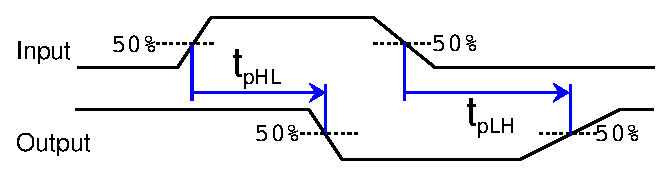
\includegraphics[scale=1.]{figuras/tiempo_retardo_tpHL-tpLH.eps}
  \caption{Retardo de propagación de un inversor}
  \label{fig:propagationDelay}
\end{figure}



\subsubsection{Mínimo retardo de propagación}

Para poder comparar la performance de distintas tecnologías, se busca un circuito que no incluya parámetros como el fan-in o fan-out, que influyen en los tiempos $t_f$, $t_r$ y $t_f$. Por ello, el circuito que es un estándar de facto para medir el tiempo de propagación, es el oscilador anillo (\emph{ring oscillator}), que es un número impar de inversores conectados en serie, con la salida conectada a la entrada. Este circuito oscilla espontaneamente, a una frecuencia de $T = 2 \times t_p \times N$, con $N$ el número de inversores en la cadena. 

Contar con esta métrica nos permitirá tener una referencia del límite inferior impuesto por la tecnología que se esté utilizando. Por ejemplo, tomemos la tecnología TSMC de 180~nm: La frecuencia de un oscilador anillo de 31 etapas es de 377,13~MHz. Es decir que el tiempo de propagación de una celda inversora en esta tecnología es $t_p = 47,8~ps$


%(TODO: Citar DIGITAL DESIGN OF SIGNAL PROCESSING SYSTEMS 5.5.1 )




%FIGURA
%(Multiplicadores, Filtros FIR, usando sumadores)


%Funcionamiento esperado: Se buscará acercarse lo mas posible a la frecuencia máxima de funcionamiento de los circuitos secuenciales para la tecnología CMOS seleccionada, que está caracterizada por la frecuencia de oscilación de un ring oscilator de 31 etapas. Lo
%mismo en cuanto a la especificación de potencia, se utilizará como referencia el número de unidad uW/MHz/gate de ese ring oscilator, que expresa la potencia de un inversor oscilando a la frecuencia máxima.




\subsection{Potencia promedio disipada}
Realizamos el análisis de potencia a lo largo de un período de tiempo $\mathrm{T}$. La potencia promedio disipada total la podemos calcular si conocemos la corriente instantánea que brinda la fuente de tensión $V_{DD}$, como podemos ver en la ecuación \ref{eq:pv}.
\begin{figure}[h]
\centering
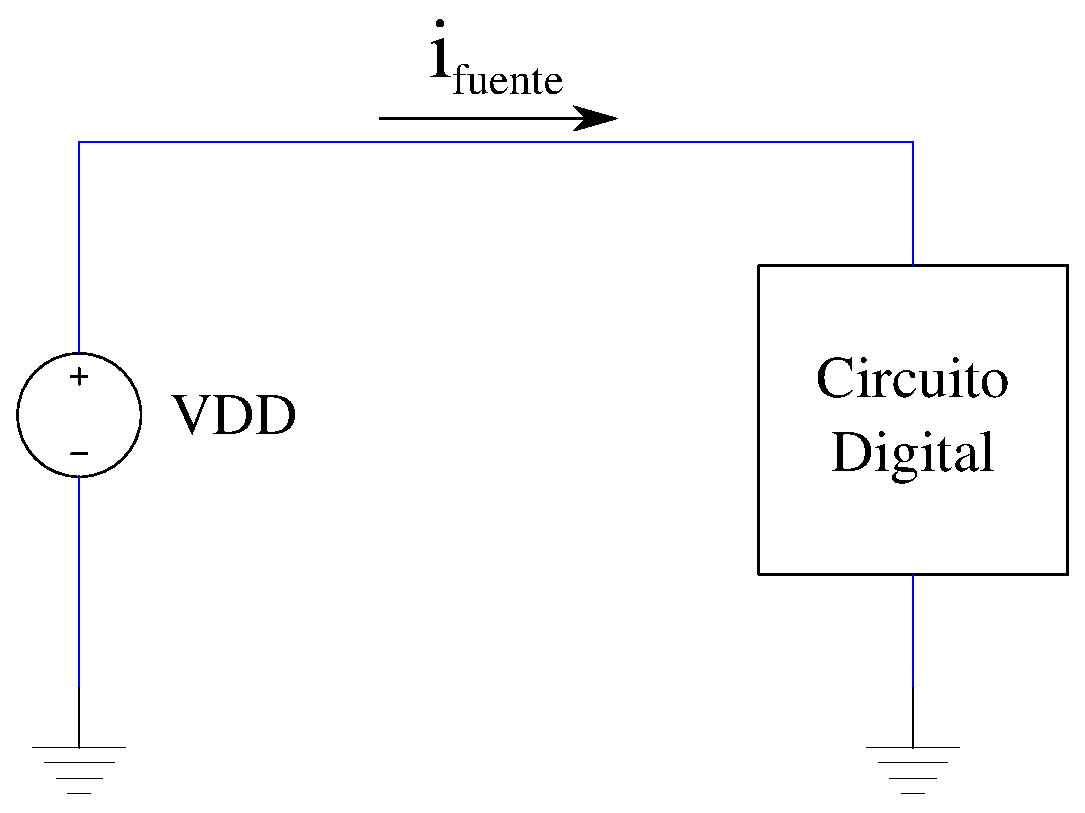
\includegraphics[scale=.5]{figuras/powerSupply.eps}
  \caption{Estimación de Potencia Promedio Disipada }
  \label{fig:powerSupply}
\end{figure}

\begin{equation}
P_{av} = \frac{1}{\mathrm{T}}\int\limits_0^T p(t)dt = \mathrm{\frac{V_{DD}}{T}}\int\limits_0^T i_{\mathrm{fuente}}(t)\mathrm{d}t 
\label{eq:pv}
\end{equation}
El período de tiempo que tomaremos para la integral es el retardo de propagación del camino crítico.

\subsection{Área}
La importancia de minimizar el área de los circuitos radica principalmente en que esta impacta fuertemente en el costo de cada \emph{die}\cite{HennessyPatterson}, ya que el costo es una función que depende de la cuarta potencia del área del circuito\cite{rabaey2003}. Además, los circuitos de menor área tienden a consumir menor energía. 


\subsection{Resumen}
A continuación resumimos en la tabla \ref{cuadro:metricas} las métricas que utilizaremos para la comparación de las distintas arquitecturas de sumadores:
\begin{table}[h] 
\centering
\begin{tabular}{@{}ll@{}}
\toprule
\textbf{Métrica}  & \textbf{Unidades} \\ \midrule
Retardo de propagación & [ns] \\	
Potencia promedio disipada & [mW] \\
Área de circuito  & [$\mu\textrm{m}^2$] \\ \bottomrule
\end{tabular}
\caption{Métricas de comparación}
\label{cuadro:metricas}
\end{table}




%Quality Metrics of a Digital Design
%Área 
%cost of die = f(die area)^4



%Background:
%Power consumption on cmos
%Dynamic Power, Static Power
%Delay in CMOS



%Glosario:

%Chip
%A tiny, thin square or rectangle that contains integrated
%electronic circuitry. Die are built in batches on wafers
%of silicon. A chip is a packaged die. Chips are also called
%processors and microprocessors. Microprocessors are the
%brains of computers, servers, communications products,
%and other digital devices

%Die: Alternate name for a chip, usually before it is packaged.
%See also Chip


%Wafer
%A thin silicon disc sliced from a cylindrical ingot. Used as
%the base material for building integrated circuits.
